% !TeX root = ./document.tex
\chapter{Reálné funkce, limita a spojitost}
Funkce z $M$ do $N$ je předpis, který každému prvku $M$ přiřadí nejvýše jeden \\ prvek z $N$
\begin{itemize}
    \item $A\subset M:f(A)=\left\{f(x); x\in A\right\}\subset N$
    \item $B\subset M:f^{-1}(B)=\left\{x\in M: f(x)\in B\right\}\subset M$
\end{itemize}

\begin{definition}[Prostá funkce, injekce, monomorfismus]\labelTheo{D-injection}
    Funkce je \textbf{prostá}, pokud
    \begin{equation}
        x\neq y \Rightarrow f(x)\neq f(y)
    \end{equation}
\end{definition}

\begin{definition}[Na funkce, surjekce, epimorfismus]\labelTheo{D-surjection}
    Funkce $f:M\rightarrow N$ je \textbf{na} (zobrazuje $M$ na $N$), pokud
    \begin{equation}
        \forall n\in\mathbb{N}~\exists m\in M: f(m)=n
    \end{equation}
    \begin{figure}[ht!]
        \begin{center}
            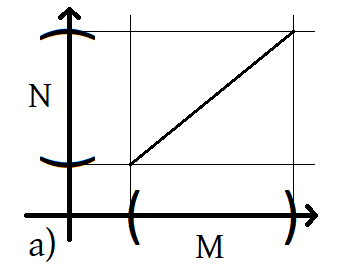
\includegraphics[width=0.4\textwidth,keepaspectratio]{../img/chapter2/surjectiveFunction.png}
            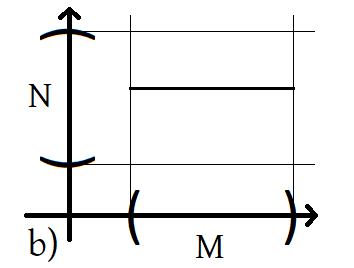
\includegraphics[width=0.4\textwidth,keepaspectratio]{../img/chapter2/surjectiveFunctionNOT.png}
            \caption{Funkce a) je na, funkce b) není.}
        \end{center}
    \end{figure}\FloatBarrier
    Př.: $\varphi$ není prostá, zobrazuje $\mathbb{R}$ na $[0,+\infty)$
    \begin{alignat}{1}
        \varphi:\mathbb{R}&\rightarrow\mathbb{R} \\
        x&\rightarrow x^2 \\
        \varphi((-1,1))&=[0,1)] \\
        \varphi^{-1}([1,4])&=[-2,-1]\cup[1,2]
    \end{alignat}
\end{definition}

\begin{definition}[Vzájemně jednoznačné zobrazení, bijekce , isomorfismus]\labelTheo{D-bijection}
    Je-li $f:M\rightarrow N$ \hyperref[D-injection]{prostá} a \hyperref[D-surjection]{na} říkáme, že je vzájemně jednoznačná
\end{definition}

Pro \hyperref[D-bijection]{vzájemně jednoznačnou funkci} lze definovat inverzní funkci:
\begin{equation}
    f_{-1}:N\rightarrow M; y\in N\rightarrow \text{jediné }x\in M: f(x)=y
\end{equation}
\[
\textbf{Pozor!}
\begin{cases}
    f^{-1} \quad\text{pro každou hodnotu zvlášť, je to množina} \\
    f_{-1} \quad\text{inverzní funkce}
\end{cases}
\]

\begin{definition}[Restrikce, zúžení]
    Je-li $f:M\rightarrow N$ a $A\subset M$: $f|_A$ nazvu restrikce (zúžení) $f$ na $A$
\end{definition}
\begin{example}
    $\varphi(x)=x^2: \varphi|_{[0,+\infty)}$ zobrazuje $[0,+\infty)$ na $[0,+\infty)$
    vzájemně jednoznačně. Lze tedy definovat $\varphi_{-1}=(\varphi|_{[0,+\infty)})_{-1}(x)=\sqrt{x}$
\end{example}    
        
\begin{definition}[Složená funkce, superpozice]
    Pro $M,N,K$ množiny a \\$f:M\rightarrow N; g:N\rightarrow K$ funkce definujeme složenou funkci
    \begin{alignat}{2}
        g\circ f: M&\rightarrow K &&\quad M\xrightarrow{f}N\xrightarrow{g}K \\
        x\in M &\rightarrow \left(g(f(x))\right) &&\quad x\rightarrow f(x)\rightarrow\left(g(f(x))\right)
    \end{alignat}
    Budeme psát: $\varphi :M\rightarrow N$ i když $\varphi(x)$ není definované $\forall x\in M$
\end{definition}

\begin{definition}[Definiční obor a obor hodnot]
    \begin{alignat}{1}
        D(\varphi)&=\left\{x\in M: f(x) \text{ je definovaná}\right\} \\
        H(\varphi)&=f\left\{D(\varphi)\right\}
    \end{alignat}
\end{definition}
\begin{example}
    \begin{equation*}
        x^{-1}: \mathbb{R}\rightarrow\mathbb{R} \quad
            D\left(x^{-1}\right)=\mathbb{R}-\left\{0\right\} \quad
            H\left(x^{-1}\right)=\mathbb{R}-\left\{0\right\}
    \end{equation*}
\end{example}

\begin{definition}[Monotónost funkce]\labelTheo{D-monotonic}
    Nechť $f:\mathbb{R}\rightarrow\mathbb{R}$; $M\subset D(f)$. Řeknu, že $f$
    \[
        \text{je}\left.%\{
        \begin{cases}
            \text{rostoucí} \\
            \text{klesající} \\
            \text{nerostoucí} \\
            \text{neklesající}
        \end{cases}
        \right\} \text{na $M$, pokud }\forall x_1,x_2\in M:x_1<x_2\Rightarrow f(x_1)\left.
        \begin{cases}
            < \\
            > \\
            \geq \\
            \leq
        \end{cases}
        \right\}f(X_2)
    \]
    \begin{figure}[ht!]
        \begin{center}
            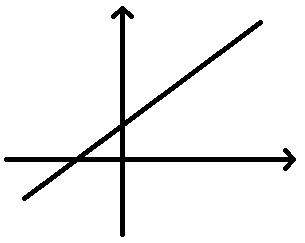
\includegraphics[width=0.24\textwidth,keepaspectratio]{../img/chapter2/monotonic1.png}
            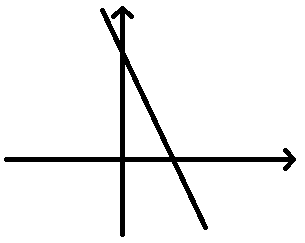
\includegraphics[width=0.24\textwidth,keepaspectratio]{../img/chapter2/monotonic2.png}
            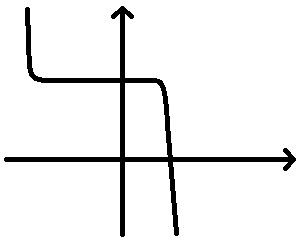
\includegraphics[width=0.24\textwidth,keepaspectratio]{../img/chapter2/monotonic3.png}
            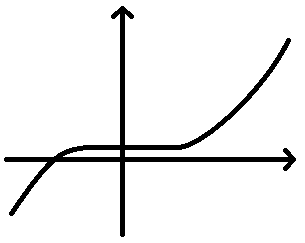
\includegraphics[width=0.24\textwidth,keepaspectratio]{../img/chapter2/monotonic4.png}
            \caption{Ilustrace.}
        \end{center}
    \end{figure}\FloatBarrier
\end{definition}

\begin{definition}[Omezenost funkce]\labelTheo{D-bounded}
    Řekněme, že $f$
    \[
        \text{je}\left.%\{
        \begin{cases}
            \text{omezená shora} \\
            \text{omezená zdola} \\
            \text{omezená}
        \end{cases}
        \right\} \text{na $M$, pokud }\exists K\in\mathbb{R}:\forall x\in M:\left.
        \begin{cases}
            f(x)<K \\
            f(x)>K \\
            \abs{f(x)}<K
        \end{cases}
        \right\}
    \]
\end{definition}

\begin{definition}[Symetrie funkce]\labelTheo{D-symetry}
    Řekněme, že $f$
    \begin{alignat}{1}
        \text{je}\left.%\{
        \begin{cases}
            \text{lichá,} \\
            \text{sudá,} \\
            \text{periodická,}
        \end{cases}
        \right\} \text{pokud}\left.
        \begin{cases}
            \forall x\in D(f) \\
            \forall x\in D(f) \\
            \exists p\in\mathbb{R}:\forall x\in D(f)
        \end{cases}
        \right\} \text{platí} \nonumber\\
        \left.
        \begin{cases}
            -x\in D(f)&\&~f(x)=-f(-x) \\
            -x\in D(f)&\&~f(x)=f(-x) \\
            x+p\in D(f)&\&~f(x)=f(x+p) 
        \end{cases}
        \right\}
    \end{alignat}
\end{definition}

Budeme zkoumat: $f:\mathbb{R}\rightarrow\mathbb{R}$ nebo $f:\mathbb{R}\rightarrow\mathbb{C}$.
Druhou variantu chápeme jako:
\begin{equation}
    f=f_1+if_2;~f_1,f_2:\mathbb{R}\rightarrow\mathbb{R}
\end{equation}

\begin{definition}[Okolí]\labelTheo{D-neighbourhood}
    Nechť $x_0\mathbb{R}, \delta\in(0,\infty)$
    \begin{itemize}
        \item kruhové okolí\quad $U(x_0,\delta):=(x_0-\delta, x_0+\delta)=
            \left\{x\in\mathbb{R}:x_0-\delta<x<x_0+\delta\right\}$ \\
            (v aj \textit{B}: ball)
        \item prstencové okolí\quad $P(x_0,\delta):=U(x_0,\delta)-\left\{x_0\right\}$
        \item pravé kruhové okolí\quad $U_+(x_0,\delta):=\left[x_0,x_0+\delta\right)$
        \item obdobně definujeme \textbf{levé kruhové okolí}, \textbf{pravé prstencové okolí} \\
            a \textbf{levé prstencové okolí}
    \end{itemize}
\end{definition}

Poznámky:
\begin{itemize}
    \item Pro $0<\delta_1<\delta_2\Rightarrow U(x_0,\delta_1)\subset U(x_0,\delta_2)$
    \item Budeme psát: „na jistém $U(x_0)$ platí\dots“, což znamená \\
        $\exists\delta>0:\forall x\in U(x_0,\delta)$ platí\dots
\end{itemize}



